\section{Hardware}
\label{hardware}


\subsection{Diseño mecánico}

El diseño del robot se ha realizado mediante el programa FreeCAD. FreeCAD, es un programa de modelado 3D paramétrico. El motivo fundamental de haber utilizado FreeCAD, es que es un programa libre. Para realizar el diseño mecánico del robot, se han tenido en cuenta los siguientes requisitos:

\begin{itemize}
	\item El robot tendrá una configuración diferencial.
	\item Poseerá una pinza que le permita recoger latas.
	\item Sus piezas deberán tener el tamaño adecuado para poder ser fabricadas en una impresora 3D de escritorio.
\end{itemize}

Siguiendo estos puntos, se ha diseñado un chasis con dos ruedas laterales. El tercer punto de apoyo se ha conseguido utilizando una canica. En la figura \ref{fig:abajo} se muestra una imagen del robot visto desde abajo, pudiendo observarse la colocación de las ruedas y de la canica en el chasis.

\begin{figure}[H]
        \centering
        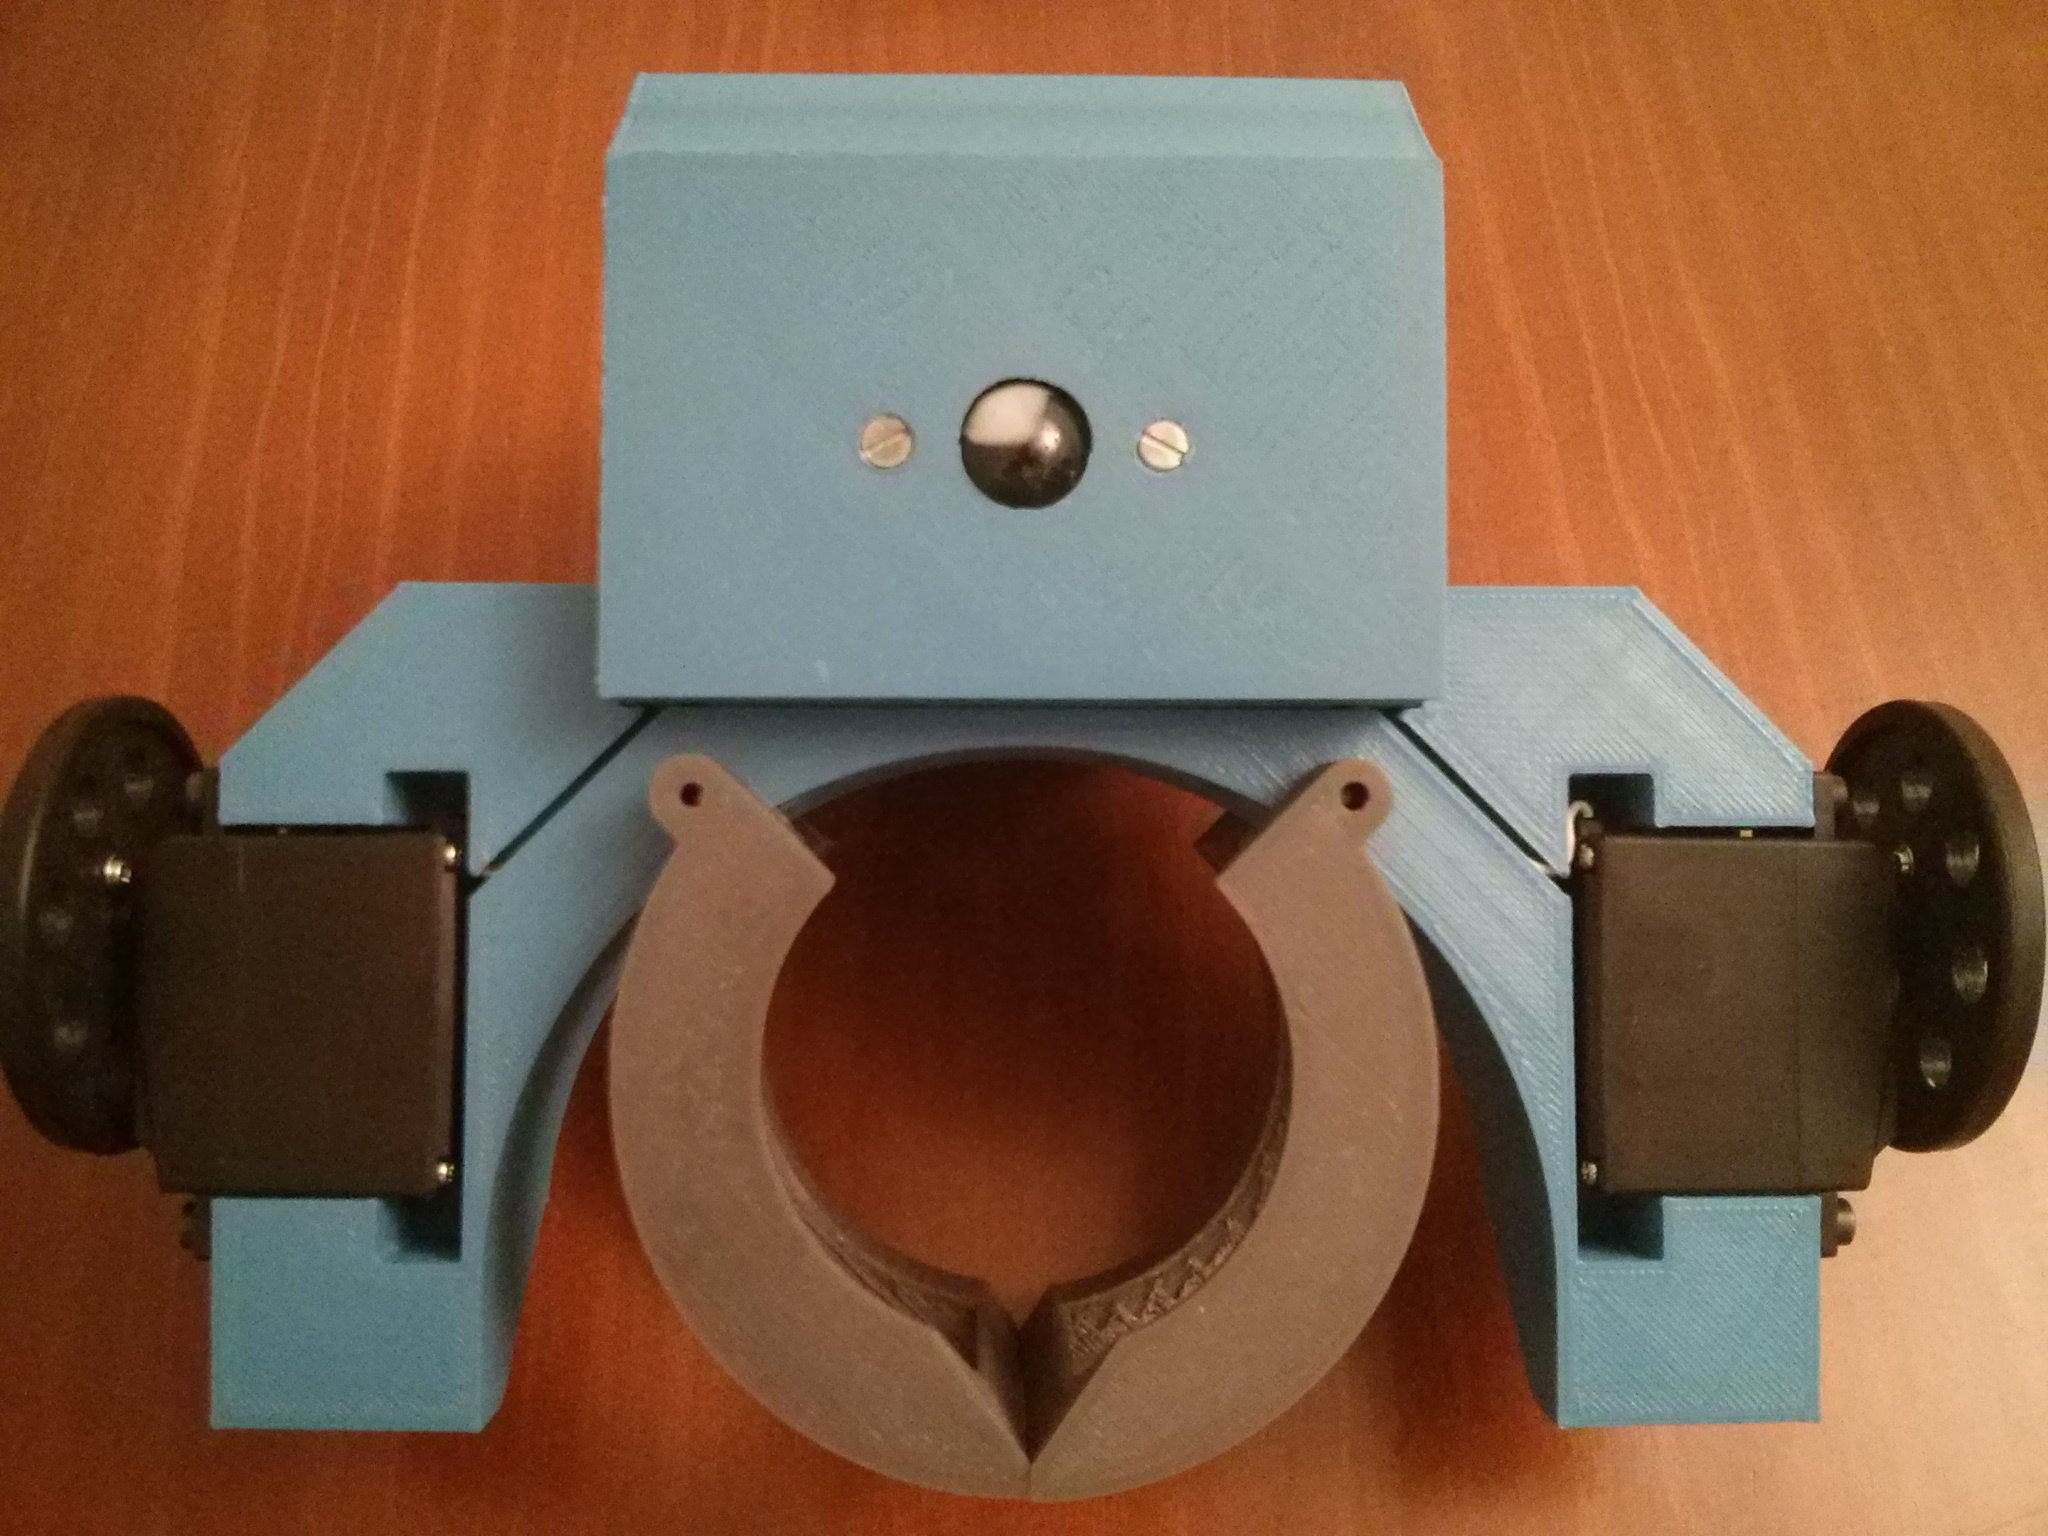
\includegraphics[width=0.4\textwidth]{images/abajo.jpg}
        \caption{Vista inferior del Beerbot}
        \label{fig:abajo}
\end{figure} 
El chasis sirve de soporte para la pinza, la cual se actuará mediante un sistema de rótulas esféricas que transmitirán el movimiento desde un servomotor. Este sistema, además de presentar una gran robustez, permite controlar de manera precisa el rango de apertura de la pinza. Dado que la pinza cumplirá únicamente la función de agarrar latas, se ha diseñado un saliente en su parte inferior que permite elevar las latas ligeramente en el momento de agarrarlas. Gracias a esto, la lata no rozará contra el suelo y el robot podrá moverse libremente. El resultado puede observarse en la figura \ref{fig:pinza}.

\begin{figure}[H]
        \centering
        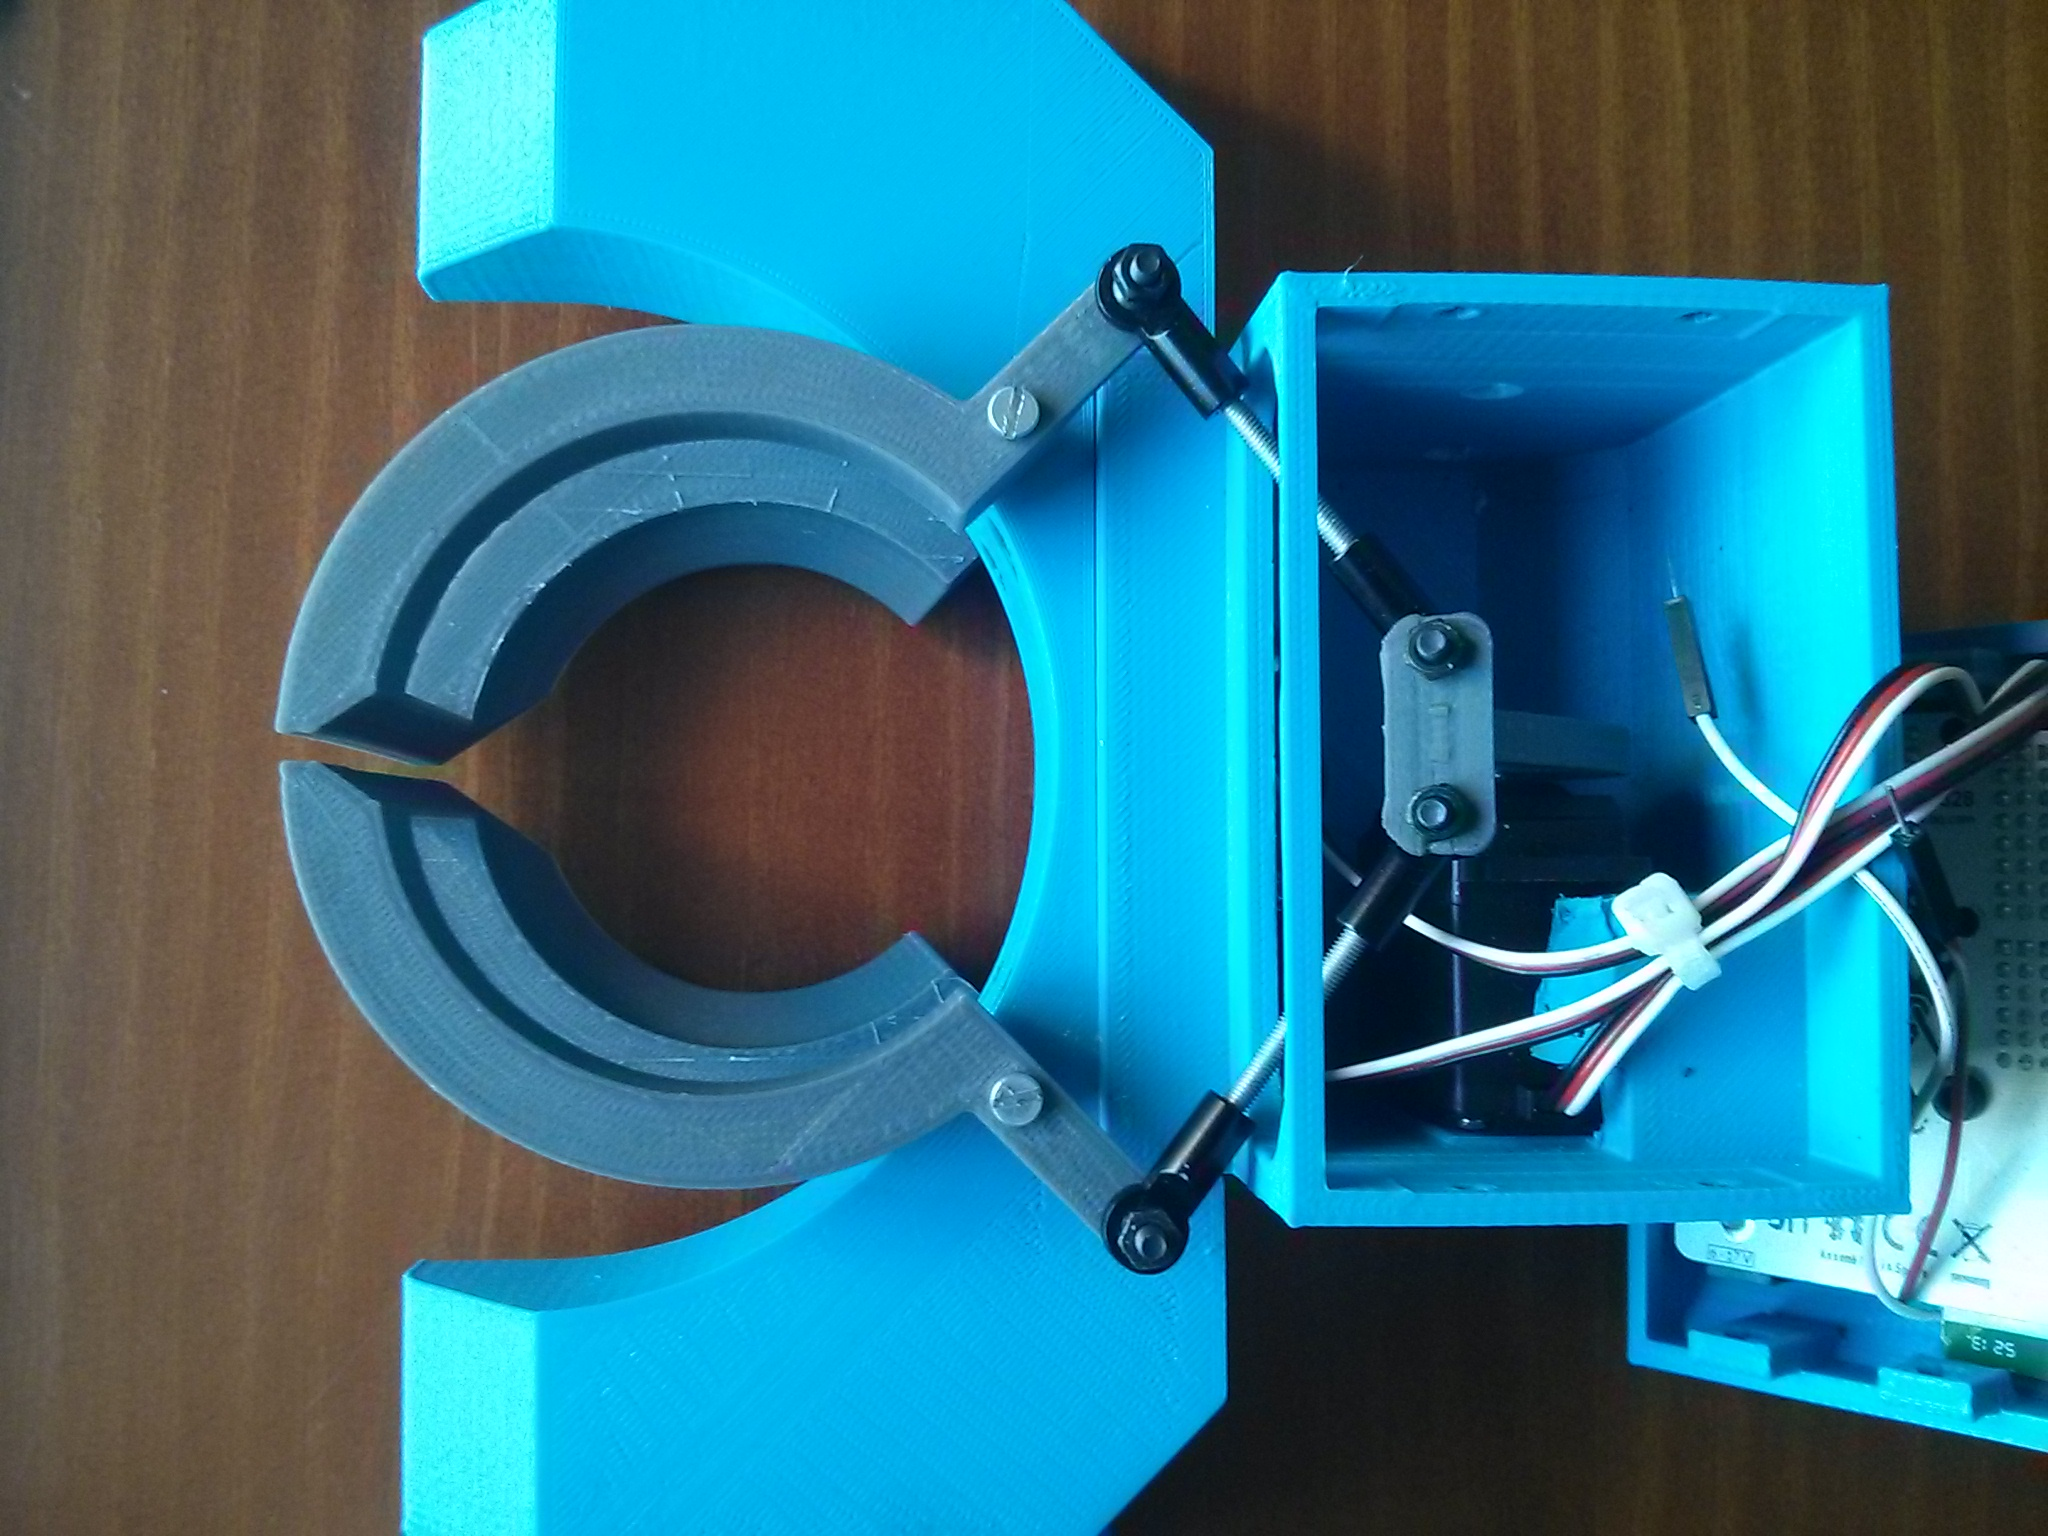
\includegraphics[width=0.4\textwidth]{images/pinzacerrada.jpg}
        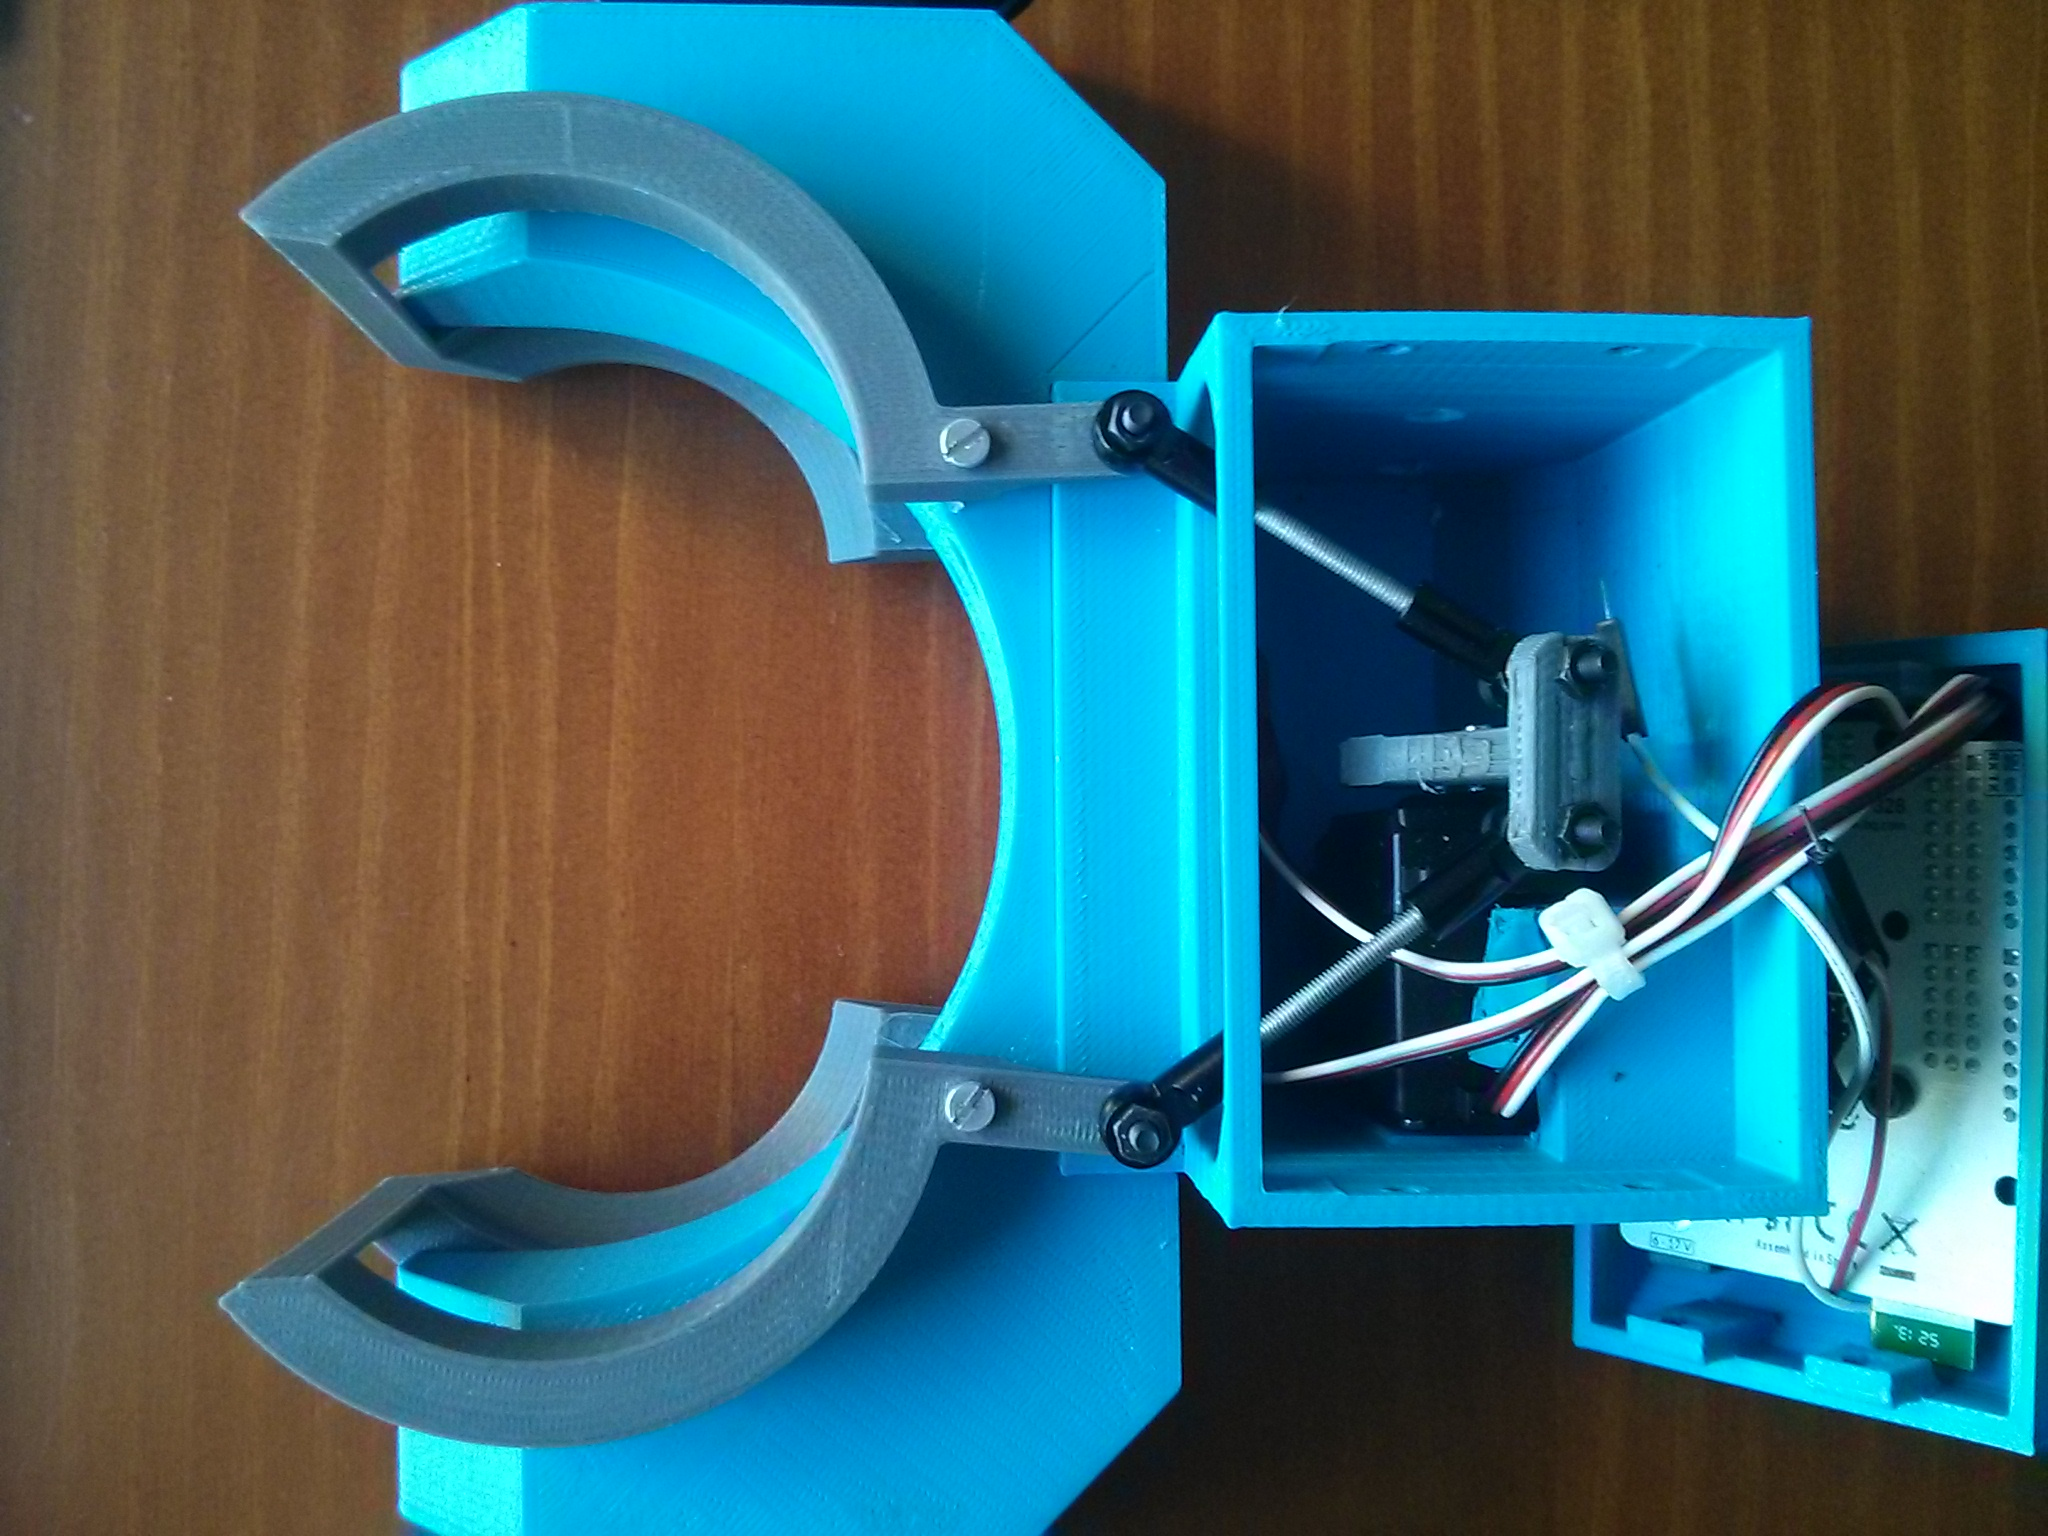
\includegraphics[width=0.4\textwidth]{images/pinzaabierta.jpg}
        \caption{Apertura de la pinza}
        \label{fig:pinza}
\end{figure}

Se han diseñado un total de ocho piezas para montar el robot. Ninguna de ellas excede en planta una superficie de 20x20cm, lo que las hace imprimibles en la mayoría de las impresoras 3D de escritorio. En este caso particular, las piezas han sido impresas en un impresora BQ Witbox. El resultado final puede observarse en la figura \ref{fig:beerbot}.

\begin{figure}[H]
        \centering
        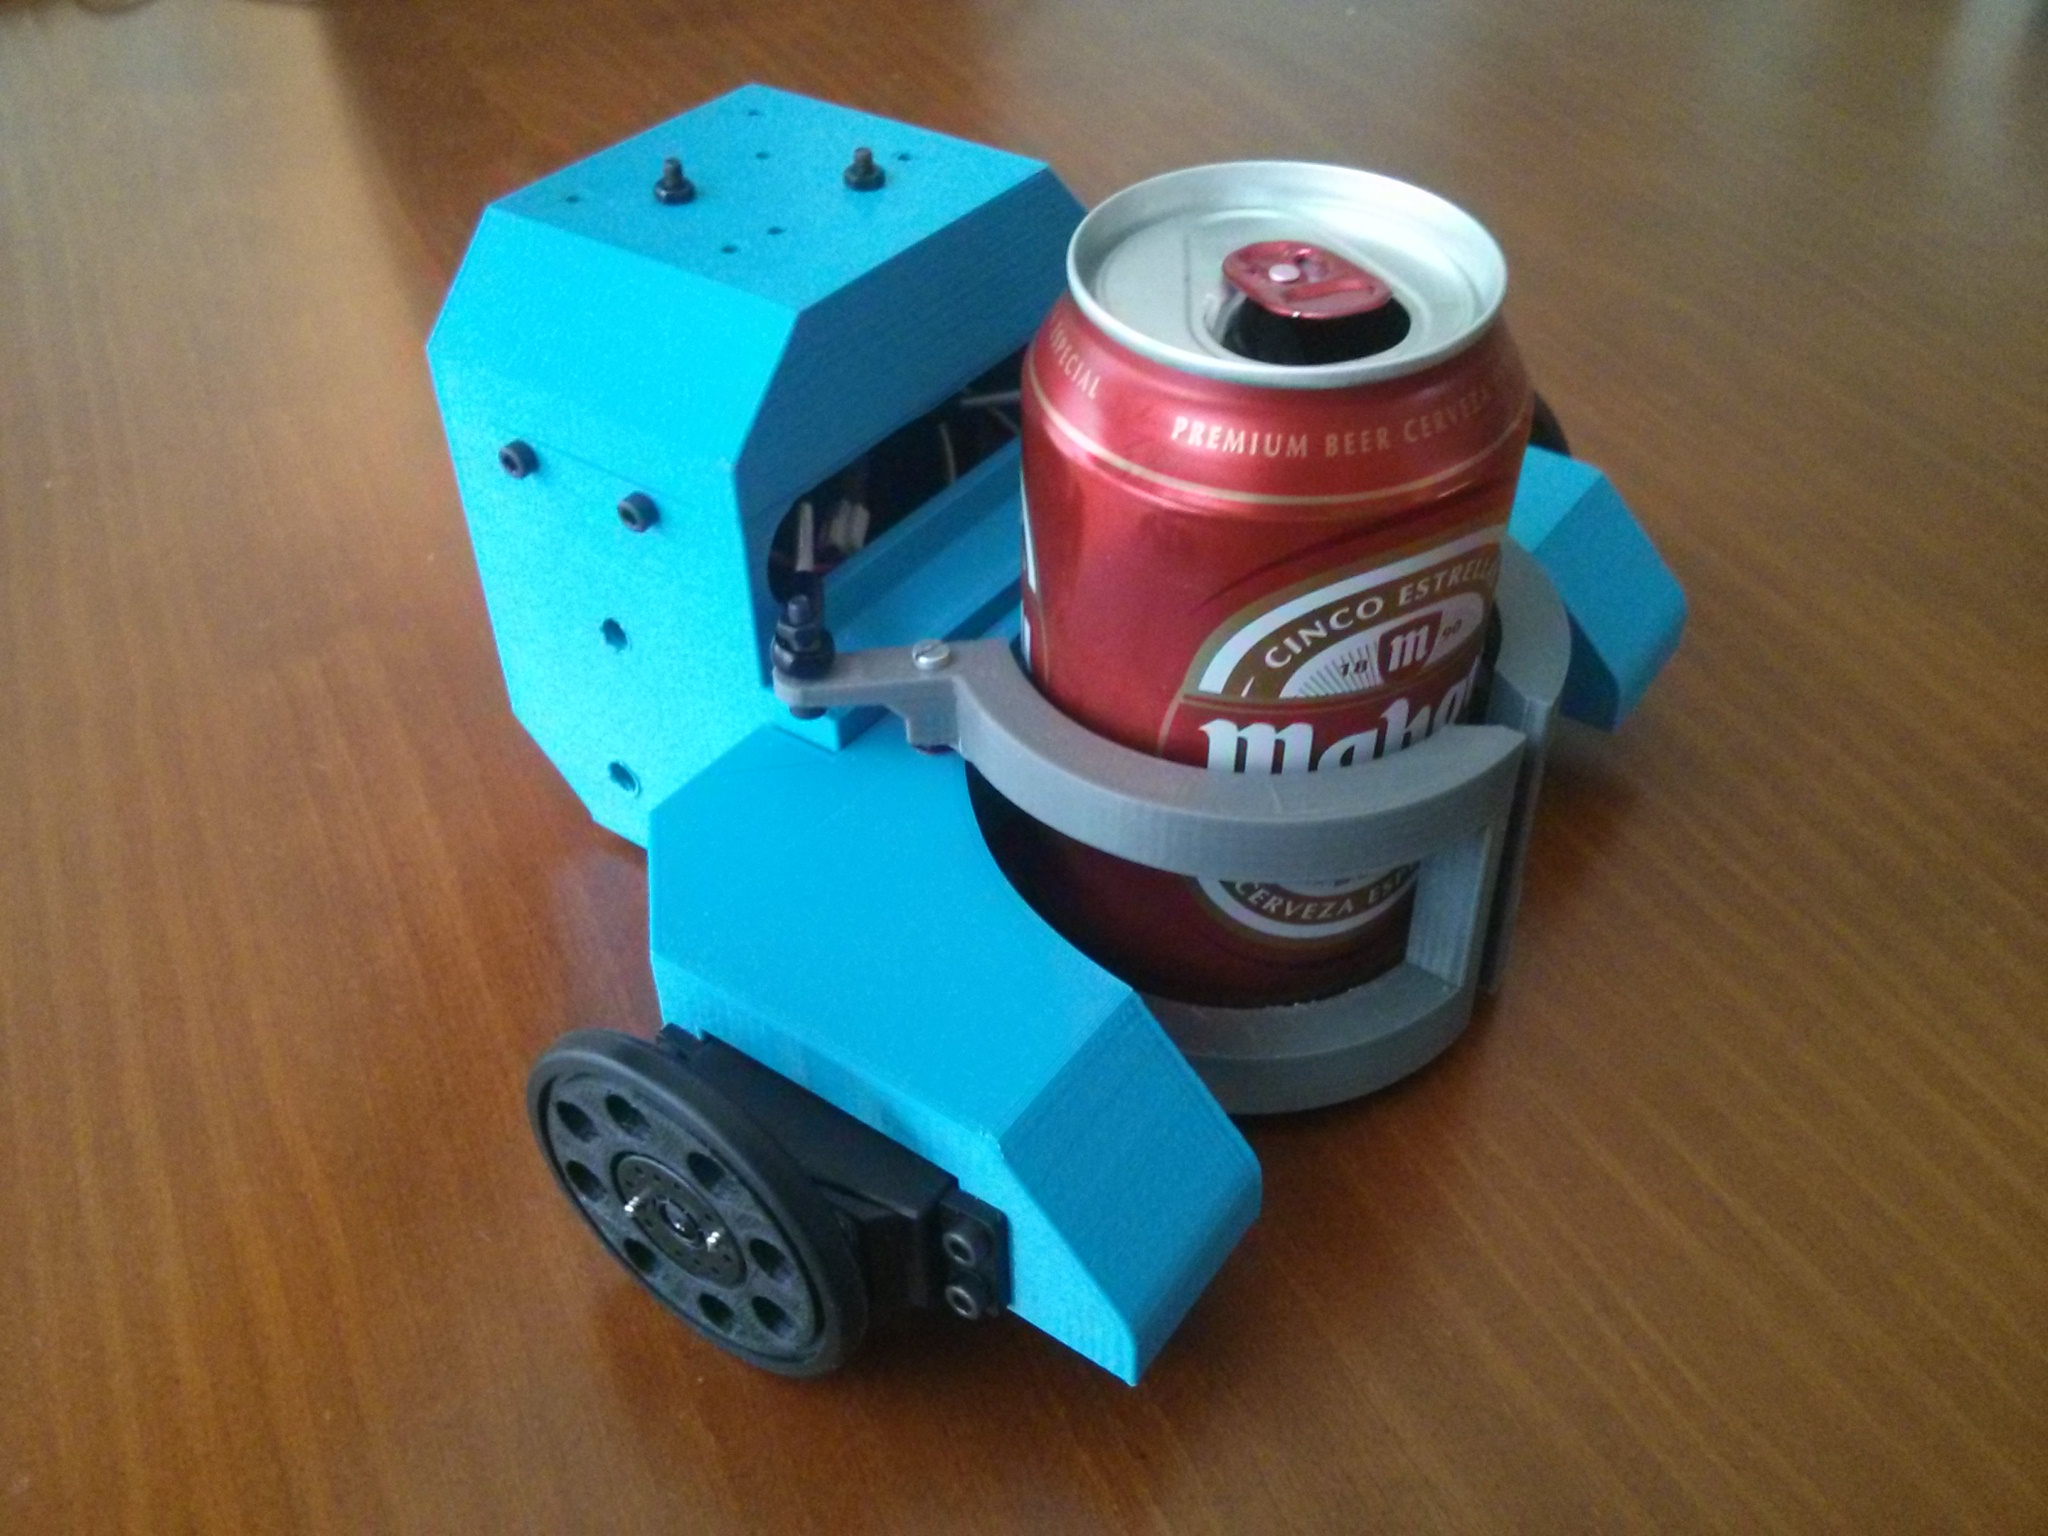
\includegraphics[width=0.4\textwidth]{images/beerbot.png}
        \caption{Beerbot ensamblado}
        \label{fig:beerbot}
\end{figure} 

\subsection{Electrónica}

El robot utiliza un controlador BQ ZUM. Esta placa está basada en el microcontrolador ATmega328. La decisión de utilizar esta placa radica en que incluye un módulo Bluetooth, así como un sistema de alimentación que permite conectar directamente a la placa los motores del robot. En la figura \ref{fig:zum} puede observarse una placa BQ ZUM.

\begin{figure}[H]
        \centering
        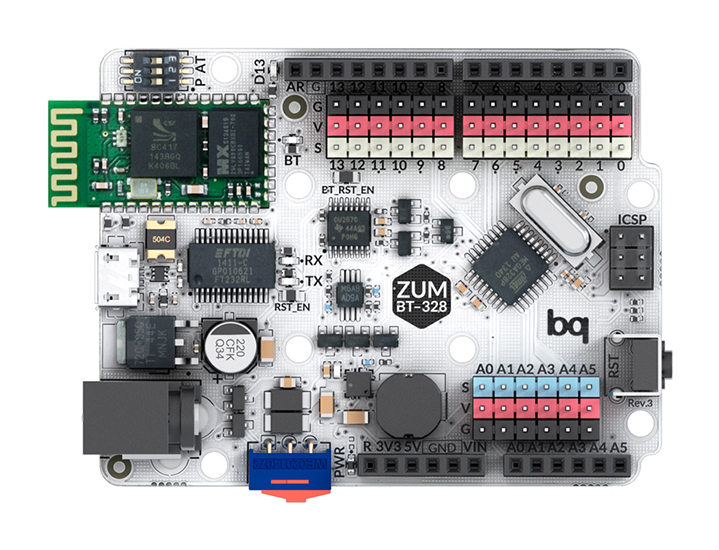
\includegraphics[width=0.4\textwidth]{images/zum.jpg}
        \caption{Placa controladora BQ ZUM}
        \label{fig:zum}
\end{figure} 

Para mover las ruedas del robot, se han utilizado dos servos de tamaño estándar de la marca Futaba, cómo el mostrado en la figura \ref{fig:futaba}. Estos servos han sido modificados para que rotasen de forma continua inutilizando el potenciómetro interno. El motivo de utilizar servos en vez de motores de corriente continua es principalmente el precio, la facilidad de controlarlos y que son fáciles de encontrar en tiendas de radiocontrol. La modificación del servo nos permite pasar de controlar el giro en posición a controlarlo en velocidad. Adicionalmente, se ha utilizado otro servo (sin modificaciones) para controlar la pinza.

\begin{figure}[H]
        \centering
        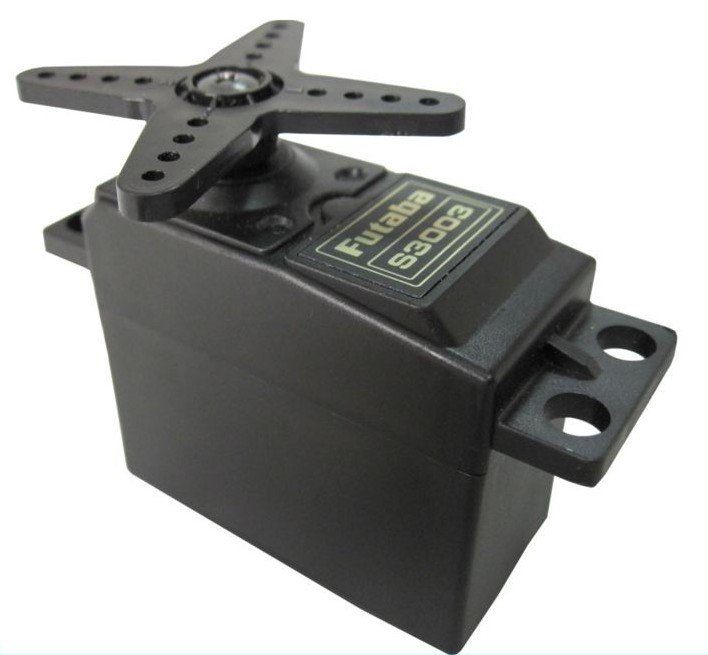
\includegraphics[width=0.4\textwidth]{images/futaba.jpg}
        \caption{Servo Futaba s3003}
        \label{fig:futaba}
\end{figure} 
En lo que a alimentación se refiere, se ha utilizado una batería de litio de dos celdas, con una tensión de 12V y una capacidad de 1000mAh. La autonomía del robot en constante movimiento es de aproximadamente 60 minutos. Dado que las pruebas realizadas no exceden los 5 minutos de duración, es una autonomía bastante razonable.

\subsection{Arquitectura del sistema}

El sistema completo, contará con tres elementos principales: el robot, una cámara y un ordenador. La cámara estará conectada al ordenador, el cual se comunicará a su vez con el robot de forma inalámbrica. En el esquema de la figura \ref{fig:arquitectura} se muestra la arquitectura completa del sistema.

\begin{figure}[H]
        \centering
        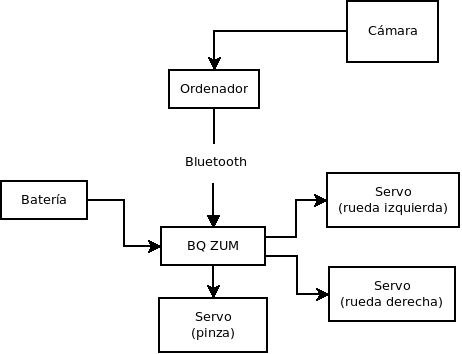
\includegraphics[width=0.6\textwidth]{images/arquitectura.jpg}
        \caption{Arquitectura hardware}
        \label{fig:arquitectura}
\end{figure} 